\subsection{Object-Oriented Analysis of Problem Domain}
In this subsection we analyse the the problem domain using the object oriented methods, with regards to how a bus system currently works. We start out by having an event table, then we explain what all the different classes contain, then we have a class diagram for the problem domain, and lastly we have a behaviour diagram.

\subsubsection{Event Table}

Bellow is an event table, it contains the classes and events of the problem domain. It was made to help figure what events the different classes are using. But first, a small story of what a typical bus driver does will be made in order to have something to loosely base the events and classes on.

The bus driver shows up for work and starts his shift. He walks over to the bus that he will be driving and inspects the exterior of the bus to figure out if anything is wrong with it. He then starts up the bus and makes sure that everything inside the bus is also working. He checks that he has enough coins to pay back people that buy the tickets with cash, and he checks that the bus is clean. After this, he drives to the first bus stop on the route. While driving around he pays attention to the traffic and objects around him and makes sure that he does not crash into any of them, furthermore he follows all the traffic laws in Denmark. When he gets close to a bus stop he checks if any of his passengers have pressed the button signalling that they want to get off at the bus stop. If one or more passengers have done that or he can see that one or more persons are waiting for the bus at the bus stop he will pull over at the bus stop and open the doors. The passengers use the middle and bottom doors to get off the bus, if they used a digital card to check in at the front door, then they use the same card to check out at the other doors. The passengers coming through the front door can as mentioned earlier use a digital card to check themselves in, they can also use cash to pay for a ticket that the bus driver prints out to them. They can also show the bus driver their bus pass, or they can show the bus driver a digital ticket on their smartphone. In case a passenger has an invalid ticket, then the passenger will be asked to buy a new ticket or be kicked off the bus. In case the passenger is in a wheelchair, has a stroller with them or a lot of baggage, then they can enter the bus using the middle door, and then go up to the bus driver at the front door and use of the aforementioned methods to get allowed to use the bus. If a passenger is misbehaving then the passenger will get kicked off the bus, and the police might be called. Once all the passengers have gotten on/off the bus the bus driver closes the doors again, uses the blinkers to signal that he is driving back into the traffic, and then drives onward to the next bus stop. Once the shift of the bus driver is over there are 2 options. Either another driver takes over and starts his shift, or he pulls up to the end station and then lets all of the remaining passengers if any off the bus. After the bus is empty the bus driver checks the inside of the bus and makes sure that the bus is clean. After the bus is cleaned he will drive the bus over to its parking spot, turn the bus off, and then end his shift and leave work.

\begin{table}[H]
\centering
\resizebox{\columnwidth}{!}{%
\begin{tabular}{|l|l|l|l|l|l|l|l|}
\hline
\diagbox{\shortstack{Events}}{Classes}& Passenger & Potential Passenger & Ticket & Bus Driver & Bus Stop & Bus Controller & Bus \\ \hline
Open/close door            &           &                     &        & x          &          & x              & x   \\ \hline
Push stop button           & x         &                     &        & x          &          & x              &     \\ \hline
See Potential Passengers   &           &                     &        & x          &          &                &     \\ \hline
Detecting obstacles        &           &                     &        & x          &          &                &     \\ \hline
Halt at bus stop           &           &                     &        & x          & x        &                & x   \\ \hline
Buy/print ticket           & x         &                     & x      & x          &          & x              &     \\ \hline
Start Bus                  &           &                     &        & x          &          & x              & x   \\ \hline
Turn bus off               &           &                     &        & x          &          & x              & x   \\ \hline
Person steps on            & x         & x                   &        &            &          &                & x   \\ \hline
Person steps off           & x         & x                   &        &            &          &                & x   \\ \hline
Maneuver the bus           &           &                     &        & x          &          & x              & x   \\ \hline
Safety handling            &           &                     &        & x          &          & x              & x   \\ \hline
Person arrives at bus stop &           & x                   &        &            & x        &                &     \\ \hline
Person leaves bus stop     &           & x                   &        &            & x        &                &     \\ \hline
Invalid ticket             &           &                     & x      & x          &          & x              &     \\ \hline
Start shift                &           &                     &        & x          &          &                &     \\ \hline
End shift                  &           &                     &        & x          &          &                &     \\ \hline
Check in                   & x         &                     & x      & x          &          & x              &     \\ \hline
Check out                  & x         &                     & x      & x          &          & x              &     \\ \hline
Starts Leaving Bus Stop            &           &                     &        & x          & x        &                & x   \\ \hline
\end{tabular}%
}
\label{event-table}
\caption{Event table}
\end{table}

\subsubsection{All Classes and What They Contain}

The list bellow is made to help explain the event table seen in table 2.1.

\begin{itemize}
\item \textbf{Passenger:}
The passenger is a person that is riding the bus. They can press the stop button when they want to get off the bus at the next bus stop. They can buy tickets from the bus driver using currency. And can both step on the bus, and step off the bus. If they have a digital ticket, then they can scan the ticket to check in and scan the ticket again to check out once they get off the bus.
\item \textbf{Potential passenger:}
A potential passenger is a person that is located at the bus stop. They can step on and on the bus similar to the passenger. A potential passenger can arrive at the bus stop and leave the bus stop again. While they are at the bus stop, the bus is required to stop at the bus stop.
\item \textbf{Ticket:}
A ticket allows the passenger to ride the bus. It can either be a digital ticket or it can be a printed ticket. It gets bought whenever a passenger pays for it. It is possible for a ticket to be invalid if it for an example has expired. It is used when the passenger checks in and when they check out.
\item \textbf{Bus driver:}
A bus driver is a person that has been hired by a company to drive the busses around a pre-defined route. He can open and close all the doors on the bus.
If one or more passengers wants to get off the bus, or if one or more potential passengers wants to get on the bus, then the bus driver stops at the bus stop. When all the passengers/potential passengers have gotten on or off bus, the bus driver closes the doors, and drives off into the main driving lane when a space is available for the bus to fit into. Whenever the bus has stopped at a bus stop because a passenger has pressed the stop button, then he can press a button to reset the stop signal. Whenever he drives towards a bus stop, the driver has to use his eyes to detect if there are any potential passengers. Whenever he is driving the bus, he has to always pay attention to detect the obstacles around him. Whenever a passenger wants to buy a ticket he takes their money, and prints the passenger a ticket. At the start off the bus drivers shift he turns the bus on, and at the end of the bus drivers shift he turns the bus off again. The bus driver uses the steering wheel to manoeuvre the bus. In case the bus driver detects an obstacle in his way he has to perform safety handling for the bus i.e. prevent collisions. It is him that checks if the tickets that the passengers use are valid or not. The bus driver starts his shift when he shows up to work, and he ends his shift when he takes off from work. When a passenger check in or out of the bus, he checks that the passenger does so correctly. 
\item \textbf{Bus stop:}
Whenever a bus halts at the bus stop they take up some space, so there is a limit to have many busses can be parked there at the same time. Whenever a potential passenger shows up at the bus stop, the bus driver will know to stop at the bus stop. There is a limited amount of seats for the potential passengers at the bus stop. A potential passenger can also leave the bus stop, and if all potential passengers leave the bus stop, then the bus driver will no longer have to stop at the bus stop for that reason. When a bus leaves the bus stop, it frees up space so that another bus can drive into the bus stop.
\item \textbf{Bus controller:}
Bus controller is all the different things the bus driver interfaces with in order to operate the bus and it's various devices. When the bus driver opens or closes the doors to the bus he does so by using some buttons, these buttons are the bus controllers. The bus controller does nothing by itself, and most of the things have already been explained in the bus driver class, so we will not go into further details with them here.
\item \textbf{Bus:}
The bus is the motor, the wheels, and the physical chassis of the bus. Similar to bus controller most of its events are handled by the bus driver and are already explained there. On top of this there are two events. One for when the passengers step onto the bus and one when the passengers steps off the bus.
\end{itemize}


\subsubsection{Class Diagram for the problem domain}

A class diagram for the problem domain can be seen in figure \ref{problem-domain-class-diagram}. This class diagram shows how the current system with a bus driver functions. This will make it easier to figure out how the class diagram for our own system should be made later on.

\begin{figure}[H]
\centering
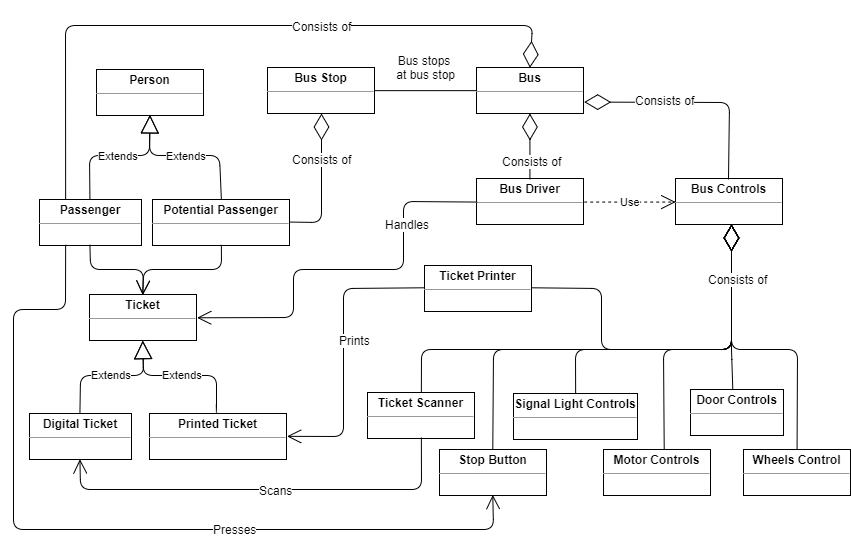
\includegraphics[scale=0.49]{Images/problem_domain_class_diagram.png}
\caption{Class diagram for the problem domain.}
\label{problem-domain-class-diagram}
\end{figure}

In figure \ref{problem-domain-class-diagram} separation becomes apparent, there are 3 different sections: the ticket part, the person part and the bus control part. The bus control part is essential to the project, since a bus cannot function without some way to control the movement of the bus. However the person part and the ticket part, are less integral to the system, since the system still has some functionality without them. For this reason we will focus the project mostly on the bus control part, which is made more complicated than the other classes because the bus control in an autonomous vehicle also has to assume the responsibilities of the bus driver.

%Our project will mirror most of what is shown in figure \ref{problem-domain-class-diagram}, however since this project will discard the bus driver, the divers responsibilities 

\subsubsection{Behaviour Diagram}

Since a central part of the project aims to produce a bus without a bus driver, the drivers responsibilities and thereby their behaviour is relevant to our project. This is why we produced a state chart diagram illustrating the behaviour of the driver, shown in figure \ref{BehaviorDiagramBusDriver}. This diagram aims to illustrate the responsibilities of the bus driver and thereby show what functionality our project has to implement.

\begin{figure}[H]
\centering
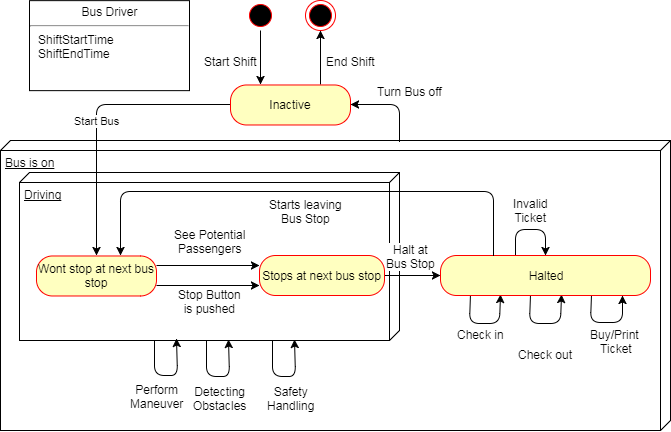
\includegraphics[scale=0.6]{Images/BehaviorDiagramBusDriver.png}
\caption{Behaviour diagram for the bus driver.}
\label{BehaviorDiagramBusDriver}
\end{figure}

In figure \ref{BehaviorDiagramBusDriver} the events handling the ticket part has been included for good measure, however since we have given bus controls a higher priority, these events can mostly be ignored. This reveals some obvious knowledge the fact that the driver is the one manoeuvring, using safety handling and detecting obstacles. This is common knowledge but maybe not as easy to implement. One of the important parts of the diagram, is the fact that the driver can be in one of two states when manoeuvring. One where the driver knows it needs to stop at the next bus stop, and one where it knows it should ignore the next bus stop. 
